\par(1)芬顿氧化技术在工业废水处理中的应用现状及趋势

芬顿氧化技术主要分为均相芬顿氧化技术与非均相芬顿氧化技术。均相芬顿氧化技术一般使用亚铁盐为催化剂,反应在液相中完成,反应过程无不同相间的传质阻力。随着对芬顿氧化机理研究的不断深入,研究者发现,通过改变芬顿试剂外部反应条件可以极大提高其氧化能力,如:紫外线照射、改变催化剂的形式等,由此形成了非均相芬顿氧化技术,如光-芬顿法\cite{liuyongdi_1994}、电-芬顿法\cite{nanjilin_2017}、铁屑-芬顿法\cite{zhangwei_1997}、超声波-芬顿法\cite{zhaochangshuang_2014}等。芬顿氧化技术首次用于废水处理是在20世纪60年代,加拿大学者H.R.Eisenhauer将芬顿氧化技术用于处理苯酚废水与烷基苯废水,效果显著,此后,芬顿氧化技术开始了其在工业废水处理中的应用。

① 焦化废水

焦化废水属于典型的有毒难降解有机废水,其所含有机污染物成分复杂,在常规生化处理过程中不能被有效去除,很难使焦化废水达标排放,常常采用预处理或深度处理技术来满足处理要求,芬顿催化氧化及其组合工艺处理焦化废水的应用越来越多。李品君\cite{liupinjun_2011}等进行了芬顿试剂+活性炭吸附处理焦化废水的试验研究,探讨芬顿氧化阶段H$_2$O$_2$投加量、Fe$^{2+}$投加量、初始pH值、反应时间和温度,以及吸附阶段吸附剂投加量和pH值等因素,研究结果表明:芬顿氧化+活性炭处理方法处理焦化废水具有良好效果,COD、氨氮和色度的去除率分别达97.74\%,83.76\%,97.33\%。刘璞\cite{liupu_2013}等采用芬顿试剂氧化+混凝沉淀法深度处理焦化生化处理二沉池出水,考察了H$_2$O$_2$投加量、H$_2$O$_2$/Fe$^{2+}$(物质的量比)、PFS(聚合硫酸铁)投加量、pH值、反应时间对TOC和COD去除效果的影响,并确定了适宜的反应条件。试验结果表明,TOC和COD去除率最高分别达到90.7\%和72.7\%,出水COD浓度达到(GB 8978-1996)《国家污水综合排放标准》一级。

② 印染废水

印染废水具有成分复杂、难降解有机物含量高、色度高、毒性大、可生化性差等特点。而芬顿试剂产生的强氧化性的·OH,能够使难生物降解的物质转变成易生物处理的物质并且能够破坏染料的发色或助色基团,而被广泛应用于印染废水的处理。杨林\cite{yanglin_2012}等人研究了铁炭微电解+芬顿试剂作用下靛蓝牛仔布印染废水的脱色和COD去除行为,微电解反应产生的Fe$^{2+}$和H原子等具有较强还原能力,能够高效还原分解废水中的有机污染物。研究结果表明:在铁炭质量比为2:1,pH值为3的条件下反应90min,铁炭微电解出水COD的去除率在49.20\%,色度去率达到80\%,BOD$_5$/COD值由0.248上升至0.436,可生化性提高;微电解出水在pH值为5,H$_2$O$_2$投加量为0.3\%条件下反应60min后,COD去除率可达84.1\%,色度去除率达90\%,\linebreak BOD$_5$/COD值上升至0.525;铁炭微电解+芬顿组合工艺COD的总去除率为87.26\%。Prabir Ghosh\cite{ghosh_electro-fenton_2012}等采用Electro-Fenton氧化工艺对两种不同的染料:亚甲基蓝和达旦黄进行降解研究,实验表明:在亚甲基蓝和达旦黄的浓度均为100mg/L,pH=3.0,电流密度为\linebreak[0] 4.31mA/cm2, Fe$^{2+}$浓度为1.18×10-5mol/L的条件下,当H$_2$O$_2$浓度分别为0.5mmol/L和1.0mmol/L时,该工艺60min后对亚甲基蓝和达旦黄的最大去除率分别为98\%和96\%。

③ 农药废水

农药废水是一类难生物降解的高浓度有毒有机废水,具有浓度高、色度深、毒性大、污染物成分复杂、难以生物降解等特点。傅学峰\cite{fuxuefeng_2011}等研究不同浓度H$_2$O$_2$、Fe$^{2+}$及pH下Cu$^{2+}$的存在对芬顿氧化处理苯酚模拟废水的苯酚去除率的影响和对\linebreak COD降解效果的影响,研究发现在苯酚浓度为250mg/L,最佳pH为3.0,\linebreak H$_2$O$_2$浓度为297.5mg/L,Fe$^{2+}$浓度为140mg/L时,苯酚的最高去除率为94.5\%;在此条件下,Cu$^{2+}$浓度为40mg/L时,苯酚最高去除率为97.7\%。梅荣武\cite{meirongwu_2012}等选用电絮凝氧化、Fenton氧化和电磁-Fenton氧化3种工艺作为草甘膦废水除磷预处理工艺,进行了比选试验,试验结果表明,芬顿氧化为草甘膦废水最佳预处理工艺:在pH=3,H$_2$O$_2$/Fe$^{2+}$=4:1的时候,Fenton工艺对TP的去除率在90\%以上。

④ 化工废水

化工废水中往往含有较多的氯代苯类、硝基苯类、酚类、多环芳烃类化合物,一般具有较高的毒性和致癌性,属典型的难降解工业有机废水。杨娟\cite{yangjuan_2012}等采用混凝-Fenton氧化-Fe$^0$还原工艺预处理高浓度硝基苯废水,发现当H$_2$O$_2$(30\%) 浓度为\linebreak[0] 6000mg/L,Fe$^{2+}$浓度为168mg/L时,氧化效率最高;聚铁混凝-Fenton氧化后的出水用Fe$^0$还原,最佳还原条件为:pH=3,Fe$^0$浓度1500mg/L。原水经聚铁混凝-Fenton氧化-Fe$^0$还原后,COD和硝基苯总去除率分别达90\%和98\%。Syukriyah Ishak\cite{ishak_optimization_2013}等利用\linebreak[0] Fenton试剂处理炼油厂废水,考察了Fe$^{2+}$投加量、Fe$^{2+}$浓度,pH值等因素对COD去除率的影响,实验在H$_2$O$_2$与Fe$^{2+}$的摩尔比为4,H$_2$O$_2$/COD比率为2.8,pH为8.46的最佳条件下,BOD$_5$/COD由0.27增加到0.44,实验前期的COD和BOD$_5$的去除率均达到90\%以上。罗九鹏\cite{luojiupeng_2011}等采用Fenton-絮凝法对化工综合废水进行研究。考察了\linebreak[0] Fenton反应时间、初始pH值、H$_2$O$_2$投加量、Fe$^{2+}$投加量、絮凝初始pH值以及絮凝剂投加量等因素对处理水质的影响。在Fenton反应时间为60min,初始pH值为3.5,H$_2$O$_2$及\linebreak[0] FeSO$_4$·7H$_2$O投加量分别为6.5mmol/L及600mg/L,絮凝初始pH值为6.5,PAM投加量为0.9mg/L的条件下,原水CODcr、浊度和色度去除率分别达到78.86\%、96.64\% 和\linebreak[0] 98.65\%,BOD$_5$/CODcr由原水的0.18左右提高到0.5以上,可生化性明显提高,为后续生化处理创造了极为有利的条件。

⑤ 制药废水

制药废水中有机污染物浓度高,毒性大,常含有大量的生物抑制剂而难于生物降解。许晓毅\cite{xuxiaoyi_fenton-_2012}等针对某医药中间体废水成分复杂,有机物浓度高,具有生物抑制性,废水可生化性差等特点,对其进行了铁碳微电解联合Fenton氧化-混凝沉淀预处理试验研究,结果表明整个处理系统对出水COD去除率达45.0\%,总磷的去除率达77.1\%,盐度去除率为24.8\%,色度去除率高达95\%,可生化性提高至0.29,为后续综合污水的生物处理提供了有利条件。黄挺\cite{huangting_2017}等利用Fe$^0$类芬顿法深度处理某制药集团经生化处理后的制药废水,研究了H$_2$O$_2$和零价铁粉投加量、pH值以及Fe$^0$的酸性改性对处理效果的影响,结果表明:COD去除率20\%时,可有效提高废水B/C。在pH值为3.0-3.5时,按H$_2$O$_2$:COD质量比为1:6进行投加,Fe$^0$与H$_2$O$_2$按4:1的摩尔比投加,反应在2h时能达到处理目标,即去除20\%COD。

⑥ 造纸废水

造纸废水中含有大量的纤维素、木质素、COD含量高。芬顿氧化法在造纸废水的研究与应用越来越多。郭鹏\cite{guopeng_2012}等采用芬顿深度氧化技术处理APMP木浆废水,实验结果效果表明,芬顿氧化法可以对碱性过氧化氢机械法制浆废水中难生化处理的有机物进行有效地降解,显著降低了废水的色度和CODcr浓度,经处理后的废水出水CODcr由原来的254mg/L-352mg/L降为38mg/L-83mg/L,色度由原来的196-325倍降为13-33倍,完全符合国家《制浆造纸工业水污染物排放标准》(GB3544-2008)。周志明\cite{zhouzhiming_2012}采用芬顿氧化法对苇浆造纸厂二级生化出水进行深度处理。探讨了废水初始pH、H$_2$O$_2$投加量、FeSO$_4$和PAM用量、反应温度和时间对COD和色度去除效果的影响,研究结果表明,当体系pH为4、H$_2$O$_2$投加量为10mmol/L、FeSO$_4$投加量为2.5mmol/L、PAM用量为0.75mg/L、反应温度为20℃和时间为40min时,COD\linebreak[0] 可降至60mg/L以下,色度去除率在90\%以上。

(2)市场同类技术比较

与其他高级氧化技术相比,芬顿氧化法具有活性高、反应速率快、适用范围广以及投资运营费用低等优点\cite{canizares_costs_2009},结合目前国内外芬顿氧化技术在难降解有机废水深度处理方面的研究及应用情况,芬顿氧化技术在工业废水深度处理领域具有很好的应用前景。目前市场上已有多家环保公司具有成熟的芬顿氧化技术,其中典型的有威水星空(北京)环境技术有限公司的非均相催化氧化技术、南京赛佳环保实业有限公司的SGE-EFP型电芬顿污水处理设备、南京神克隆科技有限公司的三相催化氧化深度水处理技术。

① 威水星空非均相催化氧化技术

针对芬顿氧化技术存在的药剂成本较高、反应pH值要求苛刻,回调pH成本高、反应过程中产生大量Fe(OH)3污泥等不足,该公司通过专效固体催化剂与高效反应器相结合的处理工艺,较好的解决了上述问题,其中用到的专效固体催化剂是将铁氧化物与锰、硅等活性激发物质进行配方复合,实现更高的活性和稳定性,促进反应过程·OH的产生,从而能更高效地降解污染物。该公司将此项技术应用于江西晨鸣纸业有限责任公司废水深度处理工艺提标改造项目,改造工程于2017年10月建成并投入运营,设计日处理水量24000m3,实际交由威水星空处理的水量在23000-24000m3,二沉池出水经非均相催化氧化流化床反应塔及后续絮凝工艺处理后,出水COD、SS与色度均达《制浆造纸工业水污染物排放标准》(GB 3544-2008)。

② 南京赛佳环保实业有限公司

该公司的SEG-EFP型电芬顿污水处理设备利用电解持续产生Fe$^{2+}$与H$_2$O$_2$,克服了传统芬顿氧化法中有机物的降解速率不均衡,先快后慢的现象,保证反应均衡,持续高效,该设备除具有芬顿氧化作用外,还有阳极氧化、阴极还原、电吸附、电气浮、电凝聚等多种作用,处理效率比传统芬顿法高,且其在反应过程中无需加入大量药剂(只需加入H$_2$O$_2$),节省了药剂费,并且处理过程清洁,不产生二次污染。该装置适用于化工、制药、农药、染料、精细化工等行业的高浓度、高色度、毒性大、难生物降解的有机废水。

③ 南京神克隆科技有限公司

该公司自主研制的三相催化氧化深度水处理技术、复合催化材料(SKL-A)和工程设备已在多家工程案例的应用中彰显了高效、低成本及稳定性好的优势,图\ref{fig1}为SKL-三相催化氧化工艺流程。

{
    \centering 
    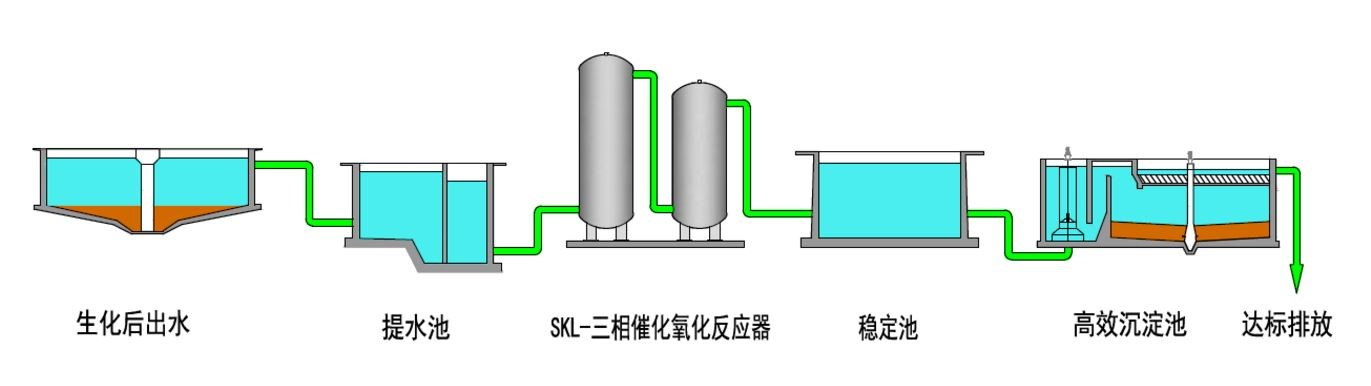
\includegraphics[width=150mm]{Img/fig1.jpg}
    \captionof{figure}{SKL-三相催化氧化工艺流程}
    \label{fig1}
}
生化出水进入双催化(催化材料A/磁化)反应系统,废水首先经过催化材料A/磁化预处理,水分子按照磁力线的方向重新排列,降低有机物活性点与药剂分子的反应屏障。再经双氧化(亚铁/氧化剂)反应系统,达到无选择地与废水中的有机污染物进行催化氧化反应、催化缩合反应。磁化显著提高催化反应速度和降解效率,能将大部分有机物分解为二氧化碳、水或简单有机物。之后进SKL-稳定池进行催化缩合反应,提高废水中残留的、难降解的、水溶性小分子污染物的混凝性、沉降性,有利于后续高效沉淀池固液分离,出水清澈透明。该工艺能快速显著降低COD,在降解COD的同时还可断开有机物分子中的发色基团,达到深度脱色目的。\par






